% This is samplepaper.tex, a sample chapter demonstrating the
% LLNCS macro package for Springer Computer Science proceedings;
% Version 2.20 of 2017/10/04
%
\documentclass[runningheads]{llncs}
%
\setcounter{secnumdepth}{5}
\usepackage{graphicx}
\usepackage{subcaption}
\usepackage{tabularx}
% Used for displaying a sample figure. If possible, figure files should
% be included in EPS format.
%
% If you use the hyperref package, please uncomment the following line
% to display URLs in blue roman font according to Springer's eBook style:
% \renewcommand\UrlFont{\color{blue}\rmfamily}

\begin{document}
	%
	\title{Predicting Rice Prices in the Philippines Using Different Machine Learning Models
	}
	%
	%\titlerunning{Abbreviated paper title}
	% If the paper title is too long for the running head, you can set
	% an abbreviated paper title here
	%
	\author{Adrian Miguel Custodio\inst{1} \and
		Rica Eunice Dordas\inst{2}\and
		Johanna Marie Quitoviera\inst{3}\and
	Ara Abigail Ambita\inst{4} }
	%
	\authorrunning{A. Custodio et al.}
	\titlerunning{Predicting Rice Prices in the Philippines Using Different Machine Learning}
	% First names are abbreviated in the running head.
	% If there are more than two authors, 'et al.' is used.
	%
	\institute{Mirasol Subd., Lapaz, Iloilo City, Iloilo\\ \email{aacustodio3@up.edu.ph} \and
		J. De Leon Street, Iloilo City, Iloilo\\
		\email{rldordas@up.edu.ph}\and
		1474 Andagao, Kalibo, Aklan\\
		\email{jpquitoviera@up.edu.ph}\and
	\email{aeambita@up.edu.ph}}
	%
	\maketitle              % typeset the header of the contribution
	%
	\begin{abstract}
	Food provides humans with nutrients and energy which is essential in surviving. In the Philippines, rice is a main staple of Filipinos where it was reported by the Philippine Statistics Authority that the average rice consumption per year would be around 118.81 kg of rice. According to Green et al. (2013), food consumption is dependent on food prices such that when.food prices increase, the food consumption decreases which causes hunger and malnutrition for poorer households in a low income country. WIth this, the study aimed to find the best machine learning model between linear regression, lasso regression, and XGBoost in making rice price predictions in the Philippines by using R2, RMSE, NRMSE, MAE, and MAPE to evaluate.  The experimental result showed that XGBoost was the model best model as it has the highest R2 value and lowest RMSE, NRMSE, MAE, and MAPE values  compared to Linear Regression and Lasso Regression. 
	
		
		
		\keywords{Linear Regression\and LASSO Regression \and XGBoost \and Food Prediction Model.}
	\end{abstract}

%
%
%
\section{Introduction}
\subsection{Background of the Study}

Food is one of the basic necessities of humans. It provides us with nutrients and energy to do our daily activities and to develop and grow which is essential in surviving. On world average, a person would consume approximately 675 kg of food per year which is equivalent to 1.85 kg per day [1]. In the Philippine context, the average person would be able to consume 855 grams per day which includes fish, rice, and vegetables [2]. Furthermore, rice is a main staple in every Filipino meal, and it was reported by the Philippine Statistics Authority that the average rice consumption per year would be around 118.81 kg which is equivalent to 325.5 grams of rice [3].\\

Rice is known as a staple food in Asian countries since it has become a part of their culture and tradition for centuries. Asia encompasses 90\% of the global consumption of rice since most of the low or middle-income countries are present here and since it gives more than 50\% of calories to a human’s body [4]. In the Philippines, every meal would not be complete without rice on the table. This attests that rice became a staple food in every family household because not only is it accessible, since a great production of rice is mostly in Asia, but also makes a person feel satiated and helps meet half of the calorie requirement that a Filipino should take.\\

According to [5], food consumption is dependent to food prices. This means that the increase of food prices will result to a decrease of food consumption which cause hunger and malnutrition for poorer households in a low income country. This is evident as the [6] reported that 95 children in the country die every day from malnutrition. Moreover, the Philippines ranked 69th out of 121 countries with a score of 14.8 which is of moderate level in the food hunger scale [7], and it is considered to be the most food-insecure country out of all the developing countries in Asia [8]. But the alarming continuous food price spikes for the second quarter of 2022 causes food consumption of those in the lower class to be minimized. 
\\

Food pricing does not only affect the consumers of the products, it also affects the agricultural and livestock industry. A study done by [9] states that “forecasting these foods’ prices play an important role in livestock and agriculture as it helps in maximizing profits and minimizing risks”. They continue on this statement by declaring that an accurate food price prediction can be utilized by the government to optimize the allocation of resources.\\

	In this research, rice prices in the Philippines is the main food commodity predicted in this study. In the process of predicting the prices of rice, different algorithms or tests were performed on the available data. The researchers aim to find the best machine learning model between linear regression, lasso regression, and XGBoost in making rice price predictions in the Philippines.

\subsection{Objectives of the Study}
The researchers of this study aims to:
\begin{enumerate}
	\item Implement and train a Linear Regression Model to predict the prices of Rice
	\item Implement and train a Lasso Regression Model to predict the prices of Rice
	 
	\item Implement and train a XGBoost Model to predict the prices of Rice
	
	\item Evaluate the 3 models and compare their scores
\end{enumerate}

\subsection{Scope and Limitations}
	The scope of the paper is to find out which among the three Machine Learning models: Linear Regression, Lasso Regression, and XGBoost can predict the price of the Rice in the country of the Philippines. It uses the dataset “Philippines - Food Prices” from The Humanitarian Data Exchange website. The researchers will mainly focus on the Rice commodity, specifically the data of : Rice (milled, superior), Rice (premium), Rice (special). Other commodities are not included in the study. The researchers also used the following tools for the study: Google Docs, Github, JupyterLab, and TeXstudio. Along with JupyterLab, the following packages were utilized: Pandas, Numpy, Sklearn, Matplotlib, and Xgboost.


\section{Methodology }
The dataset will be cleaned of empty variables and preprocessed before the training and testing stage. Then the dataset would be divided in a 75/25 split between the training and testing state, respectively. Linear Regression, Lasso Regression, and XGBoost were used on the training set to evaluate which model performs better in predicting rice prices. 

\subsection{Machine Learning Models}
\subsubsection{Linear Regression (Least Squares Approach)}
In this research, the researchers proposed to use Linear Regression in order to study the relationship of food prices across the years. Also by using this model, predictive analysis can also be done to predict the food prices in the coming years. The method of linear regression to be used in this study is the Least Squares Approach. \\

[10] states that the Least Squares method of estimation can be used to solve the problem of finding a line or curve that data points can fit in best. This paper also details the steps of the method itself:\\

In a case of a set of N pairs of observations $\{X_i, Y_i\}$ where a function relation the dependent variable Y to the independent variable X, the projection is given by the following equation,
\begin{equation}
	\hat{Y} = a + bX
\end{equation}

Wherein Y-hat is the regression line while a is the intercept and b is the gradient. The paper further states the residual $\vartheta$ for N points is the following expression:

\begin{equation}
	\vartheta = \sum_{i=1}^{N} (Y_i - \hat{Y}_i)^2 
\end{equation}

\centerline{or}

\begin{equation}
	\vartheta = \sum_{i=1}^{N} (Y_i - (a + bX_i))^2 
\end{equation}

From this relationship, partial differentiation is enforced to meet the least squares criterion. The derivative of $\vartheta$ with respect to a and b and setting them to zero obtains the following equations:

\begin{equation}
	\frac{\partial\vartheta}{\partial a} = 2Na + 2b \sum_{i=1}^{N} X_i - 2\sum_{i=1}^{N} Y_i X_i = 0
\end{equation}

\centerline{and}

\begin{equation}
	\frac{\partial\vartheta}{\partial a} = 2b \sum_{i=1}^{N} X_i^2 + 2a \sum_{i=1}^{N} X_i - 2\sum_{i=1}^{N} Y_i X_i = 0
\end{equation}

The solution to these equations then gives the least square estimates of a and b:

a = My - bMx where My and Mx are the Means of Y and X, respectively,


\begin{equation}
	b = \frac{\Sigma_{i=1}^n (Y_i - M_y)(X_i - M_x)}{\Sigma_{i=1}^n (X_i - M_x)^2}
\end{equation}


In this study, these equations are then used to produce a prediction of the dependent variable Y. In this context, the predicted value would be the food commodity prices. 

\subsubsection{Lasso Regression (Least Absolute Shrinkage and Selection Operator)}

The other learning model used by the researchers in predicting rice prices in the Philippines is the Lasso Regression.\\

According to [11], Lasso Regression algorithm or what is known as Least Absolute Shrinkage and Selection Operator is a regularization technique used for a more accurate prediction and makes the model more generalized. It eliminates insignificant variables in the data set and handles overfitting. \\

The following is the equation for the lasso regression:\\

\begin{equation}
Residual \;Sum \;of \;Squares \;+ \lambda \;(Sum \;of\;absolute \;value \;of \;magnitude \;of \;coefficients) 
\end{equation}

Where, $\lambda$ denotes the amount of shrinkage.

\subsubsection{XGBoost (Extreme Gradient Boosting)}
XGBoost was the last method used by the researchers. This is a boosting algorithm which helped improve the accuracy of the predictive models.

[12] states that XGBoost is used for approximate tree training wherein it explains cache access patterns, data compression, and build a scalable tree boosting system. This is through a sharding process which includes splitting the data  into different smaller networks. 

According to [13], the output function can be calculated with the equation:

\begin{equation}
	\hat{y}_i^T = \sum_{k=1}^{T} f_k (x_i) = \hat{y}_i^{T-1} +  f_T (x_i)
\end{equation}

 Where $\hat{y}_i^T$ is the final tree model, $ \hat{y}_i^{T-1}$ is the previously generated tree model, $f_T (x_i)$ is the newly generated tree model, and T is the total number of base tree models.

\subsection{Data Gathering}
	The data set used for this research is entitled “Philippines - Food Prices”, which was provided by the Humanitarian Data Exchange. According to its website, the dataset contains the food prices data for the Philippines, utilizing the World Food Programme Price Database (WFPPD) as its source [14]. The website further states that the WFPPD covers foods for 98 different countries and 3000 markets. \\

The dataset contains information such as the date, the food/commodity, and its prices during that day. Furthermore, it categorizes the commodities into the following: meat,fish, and eggs; vegetables and fruits; cereals and tubers; and pulses and nuts. The food is priced according to kilogram. These different commodities are then sorted by the date when their prices were logged,  dating from the 15th of January, 2000 up to the 15th of March, 2022. In addition, as to not group the same commodities that share the same date but different prices, they are grouped by region and the cities within the region. Other fields such as Price Flag and Price Type also exist to classify the prices of the commodities.\\

The dataset would be cleaned and pre-processed before it will be used in creating the training model.  Based on an article by [15], this can be done by removing the columns with missing values. For pre-processing, the currency column would be dropped since all the prices in the set are in Philippine Peso. The USD column will also be dropped as it is just the original price converted to the US dollar. Furthermore, since the columns for provinces and cities are named 'admin1' and 'admin2' respectively, they shall accordingly be renamed to their proper variables. The longitude and latitude variables are the numerical values of the provinces and cities. For the date column, they are listed in a DD/MM/YYYY format. To allow for options to reorganize data by their individual values (by day, by month, or by year), a function would be created in code to separate these values into different columns. This shall also help in the dataset training as they are now not the same string of numbers.\\

The study aimed to predict the prices of the rice and to do so, the different types of foods are to be categorized separately. Through the use of built-in features from the Pandas DataFrame, the categorical variables can be created into subcategories. These subcategories can then serve as "flags" for the data per row. The flags can be set by a yes or no identifier and due to the data being used in code, a binary identifying system will be implemented instead: 0 for No and 1 for yes. \\

Once the pre-processing is finished, the data was used for the models. The 'price' variable served as the dependent variable while the other variables were used as the independent variables. These were determined via feature selection\\

\subsection{Evaluation and Metrics}

Since the research used linear regression, the following metrics will be used to evaluate the model in terms of its accuracy:

\subsubsection{Coefficient of Determination (R Squared)}

R squared is used to determine how well the data fit the regression model.The higher the value of R2, the better the model fits the data. 

\begin{equation}
	R^2 = 1- \frac{Unexplained \;Variation}{Total \; Variation} = \frac{ \sum_{i=1}^{N} (\hat{y}_i- y_i)^2  }{ \sum_{i=1}^{N} (y_i - \hat{y}_i)^2 }
\end{equation}

\subsubsection{Root Mean Squared Error (RMSE)}
Mean Squared Error (MSE) is used to find out how the predictive values are closer to the actual values based on the standard deviation of the residuals. As the value is closer to zero, the higher the accuracy of the model. 

\begin{equation}
	RMSE = \sqrt{\frac{\sum_{i=1}^{N} (Predicted_i - Actual_i)^2}{N}}
\end{equation}

\subsubsection{Mean Absolute Percentage Error (MAPE)}
Since the dataset is large, Mean Absolute Percentage Error is also used to measure the accuracy of the forecast to include the outliers. This calculates and returns the percentage error.

\begin{equation}
	MAPE = \frac{1}{n} \sum_{i=1}^{N} \Bigg | \frac{Actual-Forecast\; value}{Actual\;value} \Bigg |
\end{equation}

\section{Results and Discussion}
This chapter discusses the results of the tests done on which among the three models have made the closest forecast on the prices of rice.

\subsection{Linear Regression}
\begin{figure}
	\begin{subfigure}{.5\textwidth}
		\centering
		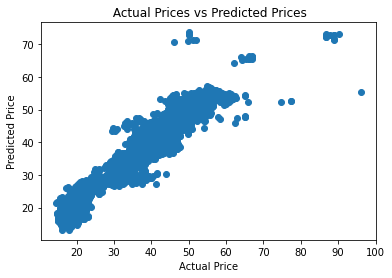
\includegraphics[width=.8\linewidth]{FIGURES/lin_train1.png}

	\end{subfigure}%
	\begin{subfigure}{.5\textwidth}
		\centering
		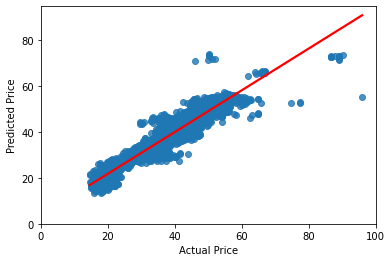
\includegraphics[width=.8\linewidth]{FIGURES/lin_train2.png}

	\end{subfigure}
	\caption{Scatter Plot of Rice Training Data using Linear Regression}
\end{figure}

Figure 1 displays the predicted prices to the actual prices of the Rice training set that was put through the linear regression model. The model produced an $R^2$ score of ~90\%, a RMSE value of ~13.46, a Normalized RMSE value of ~0.17, a MAE value of ~2.64, and a MAPE value of ~7.5\%

\begin{figure}
	\begin{subfigure}{.5\textwidth}
		\centering
		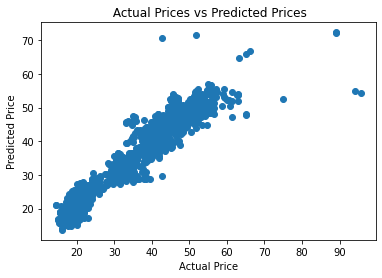
\includegraphics[width=.8\linewidth]{FIGURES/lin_test1.png}
		
	\end{subfigure}%
	\begin{subfigure}{.5\textwidth}
		\centering
		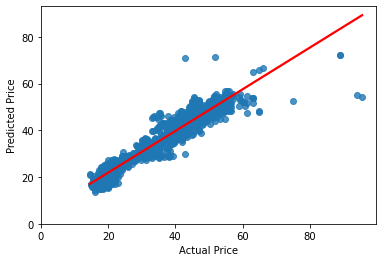
\includegraphics[width=.8\linewidth]{FIGURES/lin_test2.png}
		
	\end{subfigure}
	\caption{Scatter Plot of Rice Testing Data using Linear Regression}
\end{figure}

Figure 2 displays the predicted prices to the actual prices of the Rice testing set that was put through the linear regression model. The model produced an $R^2$ score of ~89.94\%, a RMSE value of ~15.68, a Normalized RMSE value of ~0.19, a MAE value of ~2.68, and a MAPE value of ~7.6\% \\

The results above show that the linear regression model can be considered an acceptable model as it had the $R^2$ error score of nearly 90\% for both its training and testing datasets. It also shows that it has an RMSE value 15.68, which in this context is the PHP15.68 in the range of PHP14.52 - PHP95.97. It isn’t the best distance between predicted and actual values. Lastly, it has the MAPE value of ~7.6\%, which shows good promise as the forecast values are closer to the actual values.


\subsection{LASSO Regression}
\begin{figure}
	\begin{subfigure}{.5\textwidth}
		\centering
		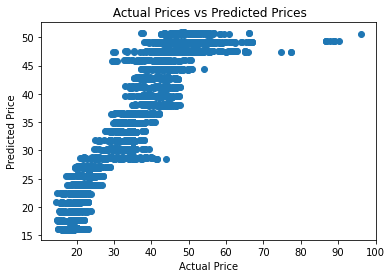
\includegraphics[width=.8\linewidth]{FIGURES/lass_train1.png}
		
	\end{subfigure}%
	\begin{subfigure}{.5\textwidth}
		\centering
		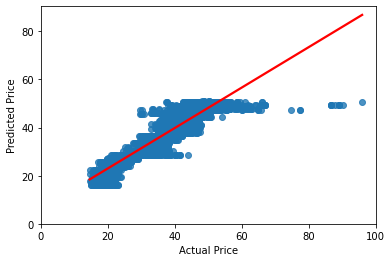
\includegraphics[width=.8\linewidth]{FIGURES/lass_train2.png}
		
	\end{subfigure}
	\caption{Scatter Plot of Rice Training Data using LASSO Regression}
\end{figure}

Figure 3 displays the predicted prices to the actual prices of the Rice training set that was put through the lasso regression model. The model produced an $R^2$ score of ~85\%, a RMSE value of ~21.46, a Normalized RMSE value of ~0.26, a MAE value of ~3.24, and a MAPE value of ~8.8\%

\begin{figure}
	\begin{subfigure}{.5\textwidth}
		\centering
		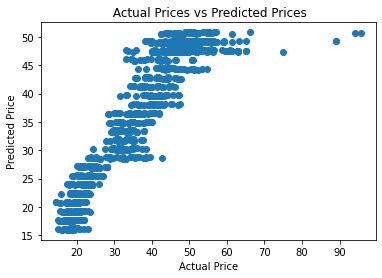
\includegraphics[width=.8\linewidth]{FIGURES/lass_test1.png}
		
	\end{subfigure}%
	\begin{subfigure}{.5\textwidth}
		\centering
		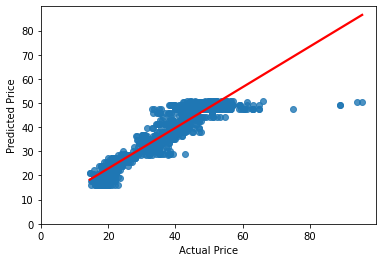
\includegraphics[width=.8\linewidth]{FIGURES/lass_test2.png}
		
	\end{subfigure}
	\caption{Scatter Plot of Rice Testing Data using LASSO Regression}
\end{figure}

Figure 4 displays the predicted prices to the actual prices of the Rice testing set that was put through the lasso regression model. The model produced an $R^2$ score of ~85\%, a RMSE value of ~22.70, a Normalized RMSE value of ~0.27, a MAE value of ~3.25, and a MAPE value of ~8.8\% \\

The results of the lasso regression model could be considered as a viable model as it got an $R^2$ score of 85\%. Its MAPE value of ~8.8\% also gives it enough merit for forecasting future possible prices. Though its RMSE value of 22.70 is not as ideal for it is a sizable distance between predicted and actual values.

\subsection{XGBoost}
\;
\begin{figure}
	\begin{subfigure}{.5\textwidth}
		\centering
		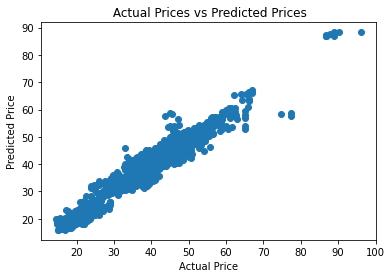
\includegraphics[width=.8\linewidth]{FIGURES/xgb_train1.png}
		
	\end{subfigure}%
	\begin{subfigure}{.5\textwidth}
		\centering
		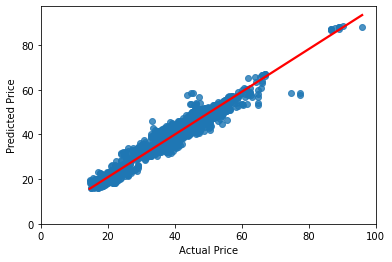
\includegraphics[width=.8\linewidth]{FIGURES/xgb_train2.png}
		
	\end{subfigure}
	\caption{Scatter Plot of Rice Training Data using XGBoost}
\end{figure}

Figure 5 displays the predicted prices to the actual prices of the Rice training set that was put through the XGBoost model. The model produced an $R^2$ score of ~96\%, a RMSE value of ~5.46, a Normalized RMSE value of ~0.07, a MAE value of ~1.72, and a MAPE value of ~4.8\%.

\begin{figure}
	\begin{subfigure}{.5\textwidth}
		\centering
		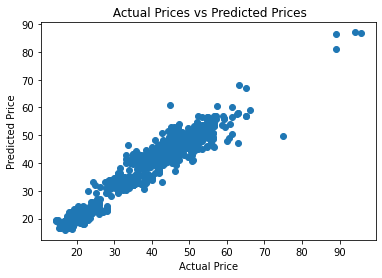
\includegraphics[width=.8\linewidth]{FIGURES/xgb_test1.png}
		
	\end{subfigure}%
	\begin{subfigure}{.5\textwidth}
		\centering
		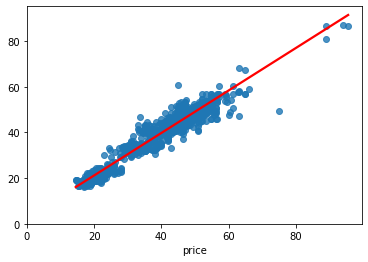
\includegraphics[width=.8\linewidth]{FIGURES/xgb_test2.png}
		
	\end{subfigure}
	\caption{Scatter Plot of Rice Testing Data using XGBoost}
\end{figure}

Figure 6 displays the predicted prices to the actual prices of the Rice testing set that was put through the XGBoost model. The model produced an $R^2$ score of ~93\%, a RMSE value of ~0.93, a Normalized RMSE value of ~0.12, a MAE value of ~2.22, and a MAPE value of ~6.1\%. \\

The XGBoost model results show good results on its evaluation scores across both training and testing sets. The $R^2$ score of both ~96\% and ~93\% makes it so that most of the values are close to the regression line. Its RMSE values are also both less than 10. Its MAPE value of between 4\% - 6\% is a good result to describe its forecasting capabilities.\\

Collectively, it is observed the training data of the models have gotten better evaluation scores than their testing datasets. 

\subsection{Data Visualization}
The graphs below show the visualization of Tables 1 and 2. It mainly compares the evaluation methods’ scores of $R^2$, RMSE, and MAPE of the training and testing datasets among the three regression models used in this paper.

\begin{table}[h!]
	\caption{Table of Evaluation Scores of Training Sets}
	\centering
	\begin{tabular}{||c c c c||} 
		\hline
		 & $R^2$ & NRMSE & MAPE \\ [0.5ex] 
		\hline\hline
		Linear Regression & 0.906750 & 0.165327 & 0.075292\\ 
		LASSO Regression & 0.851363 & 0.263526 & 0.088143\\
		XGBoost & 0.961006 & 0.069134 & 0.048905\\[1ex] 
		\hline
	\end{tabular}
\end{table}

\begin{table}[h!]
	\caption{Table of Evaluation Scores of Testing Sets}
	\centering
	\begin{tabular}{||c c c c||} 
		\hline
		& $R^2$ & NRMSE & MAPE \\ [0.5ex] 
		\hline\hline
		Linear Regression & 0.899144 & 0.192580 & 0.076494\\ 
		LASSO Regression & 0.854007	& 0.278765 & 0.088606 \\
		XGBoost & 0.938575 & 0.117288 & 0.060981\\[1ex] 
		\hline
	\end{tabular}
\end{table}

\subsubsection{$R^2$}
\;
\begin{figure}
	\begin{subfigure}{.5\textwidth}
		\centering
		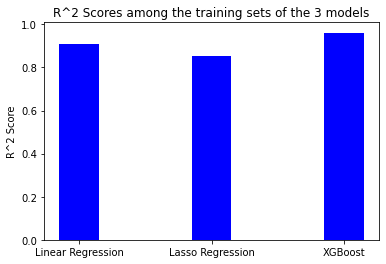
\includegraphics[width=.8\linewidth]{FIGURES/train_r2.png}
		
	\end{subfigure}%
	\begin{subfigure}{.5\textwidth}
		\centering
		\includegraphics[width=.8\linewidth]{FIGURES/test_r2.png}
		
	\end{subfigure}
	\caption{$R^2$ Error Scores of the Three Models’ Training and Testing Sets}
\end{figure}

In the figures, $R^2$ scores are ideally better the higher they are. Among the three, Lasso regression had the lowest percentage with ~85\% for both datasets. XGBoost has the highest percentage (~93\% and ~96\%) and is the most accurate with its predictions fitting in the regression line.

\subsubsection{Normalized Root Mean Squared Error}
\;
\begin{figure}
	\begin{subfigure}{.5\textwidth}
		\centering
		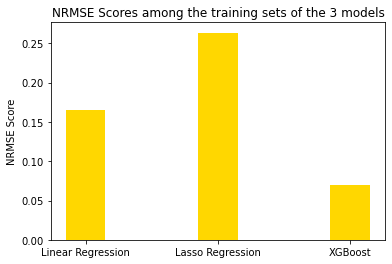
\includegraphics[width=.8\linewidth]{FIGURES/train_NRMSE.png}
		
	\end{subfigure}%
	\begin{subfigure}{.5\textwidth}
		\centering
		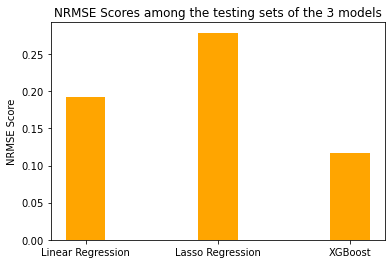
\includegraphics[width=.8\linewidth]{FIGURES/test_NRMSE.png}
		
	\end{subfigure}
	\caption{NRMSE Scores of the Three Models’ Training and Testing Sets }
\end{figure}

For Root Mean Squared Error, a comparison amongst scores on which one’s closer to 0 would determine a better performing model. The data was normalized to better show the difference between the models. With that, a big gap between the highest and lowest models is shown. This means that XGBoost, compared to the other two models, has the lowest distance between its predicted values to the actual price values.

\subsubsection{Mean Absolute Percentage Error}
\;
\begin{figure}
	\begin{subfigure}{.5\textwidth}
		\centering
		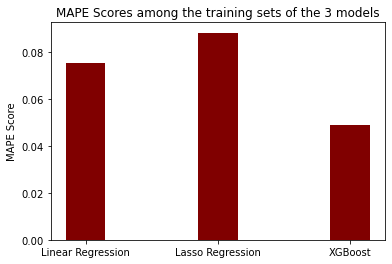
\includegraphics[width=.8\linewidth]{FIGURES/train_MAPE.png}
		
	\end{subfigure}%
	\begin{subfigure}{.5\textwidth}
		\centering
		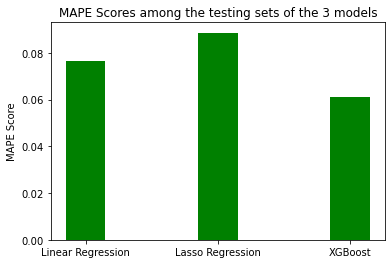
\includegraphics[width=.8\linewidth]{FIGURES/test_MAPE.png}
		
	\end{subfigure}
	\caption{MAPE Scores of the Three Models’ Training and Testing Sets}
\end{figure}

Much akin to the RMSE scores, the Mean Absolute Percentage Error (MAPE) is used for comparison with other models on which one can attain the lowest percentage. While all three models did well in their predictions as they are all lower than 10\%, XGBoost still is the best performing model with a score of between 4\% - 6\%.

\subsection{Feature Selection}
\begin{figure}
	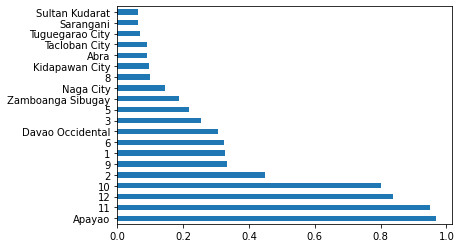
\includegraphics[width=\textwidth]{FIGURES/feature_select.png}
	\caption{Feature Selection from Pre-Processing} \label{fig1}
\end{figure}
	The original dataset, consisting of 107,354 rows and 15 columns. Due to the limitations of the study, the dataset was trimmed to where the commodities are: Rice (milled, superior), Rice (premium), Rice (special). This resulted in 5149 rows. Since most of the variables are categorical, dummy variables were created to have the value of 1 or 0. This resulted in a huge number of columns. Scikit-learn’s feature selection package was utilized to find the features that were significant enough to be used for the actual regression tests.The following columns were kept: Month, Market, and District. 


\section{Conclusion}
The study used 3 models namely Linear Regression, Lasso Regression, and XGBoost to predict the rice prices in the Philippines. $R^2$, RMSE, NRMSE, MAE, and MAPE were the metrics used to evaluate which among the 3 models will be the best to use for prediction.\\

The experimental result showed that XGBoost was the model that provided the best accuracy values. It has the highest $R^2$ value and lowest RMSE, NRMSE, MAE, and MAPE values  compared to Linear Regression and Lasso Regression. \\

With this, the model can be beneficial in predicting the rice prices in the coming years. The model determined that as the year progresses, the rice price also increases. This can help the government implement policies on how to manage the price increase of rice as this is a food staple of the Filipinos and at the same time maximize profit. This can also help the people prepare their expenses as they have an idea on the expected prices.\\

For future recommendations, other researchers can implement other models to know whether they will have better accuracy results. Also, the models can be used in other food categories in the dataset such as predicting the prices for meat, fish, and vegetables. \\


%
% ---- Bibliography ----
%
% BibTeX users should specify bibliography style 'splncs04'.
% References will then be sorted and formatted in the correct style.
%
% \bibliographystyle{splncs04}
% \bibliography{mybibliography}
%
\begin{thebibliography}{20}
	
	\bibitem{ref1}
	Good Seed Ventures. (2021, December 2). Worldwide Food Consumption Per Capita. Good Seed Ventures. https://goodseedventures.com/worldwide-food-consumption-per-capita-2/
	
	\bibitem{ref2}
	Gavilan, J. (2015, March 27). More Filipinos eat less – survey. RAPPLER. https://www.rappler.com/moveph/88070-more-filipinos-eat-less-national-nutrition-survey/
	
	
	\bibitem{ref3}
	
	DA Communications Group. (2020, May 12). Rice supply adequate for 2020. Official Portal of the Department of Agriculture. https://www.da.gov.ph/rice-supply-adequate-for-2020/
	
	\bibitem{ref4}
	IPINOY. (2020, July 25). Why is Rice the Staple Food in Many Asian Countries? | Agripinoy.net. AGRIPINOY.NET. https://agripinoy.net/why-is-rice-the-staple-food-in-many-asian-countries/
	
	\bibitem{ref5}
	Green, R., Cornelsen, L., Dangour, A. D., Turner, R., Shankar, B., Mazzocchi, M., \& Smith, R. D. (2013). The effect of rising food prices on food consumption: systematic review with meta-regression. BMJ, 346(jun17 1), f3703–f3703. https://doi.org/10.1136/bmj.f3703
	
	
	\bibitem{ref6}
UNICEF Philippines. (2014). Child survival. Unicef.org. https://www.unicef.org/philippines/child-survival
	
	
	
	\bibitem{ref7}
	Global Hunger Index. (2022). Philippines. Global Hunger Index (GHI) - Peer-Reviewed Annual Publication Designed to Comprehensively Measure and Track Hunger at the Global, Regional, and Country Levels. https://www.globalhungerindex.org/philippines.html

	
	
	\bibitem{ref8}
	Nguyen, T. (2022, July 13). Why the Philippines Is So Vulnerable to Food Inflation. Carnegie Endowment for International Peace. https://carnegieendowment.org/2022/07/13/why-philippines-is-so-vulnerable-to-food-inflation-pub-87467
	
	\bibitem{ref9}
		Wibowo, A., Yasmina, I., \& Wibowo, A. (2021). Food Price Prediction Using Time Series Linear Ridge Regression with The Best Damping Factor. Advances in Science, Technology and Engineering Systems Journal, 6(2), 694–698. https://doi.org/10.25046/aj060280
	
	
	\bibitem{ref10}
	Agbachi, C. P. E. (2016). Optimisation of Least Squares Algorithm: A Study of Frame Based Programming Techniques in Horizontal Networks. International Journal of Mathematics Trends and Technology, 37(3), 190–198. https://doi.org/10.14445/22315373/ijmtt-v37p526
	
	\bibitem{ref11}
	
	Kumar, D. (2021, October 31). What is LASSO Regression Definition, Examples and Techniques. GreatLearning. https://www.mygreatlearning.com/blog/understanding-of-lasso-regression/
	
	\bibitem{ref12}
	Chen, Tianqi \& Guestrin, Carlos. (2016). XGBoost: A Scalable Tree Boosting System. 785-794. 10.1145/2939672.2939785. 
	
	
	\bibitem{ref13}
	Mo, Hao \& Sun, Hejiang \& Liu, Junjie \& Wei, Shen. (2019). Developing window behavior models for residential buildings using XGBoost algorithm. Energy and Buildings. 205. 109564. 10.1016/j.enbuild.2019.109564.
	
	\bibitem{ref14}
	Humanitarian Data Exchange. (2022, November 22). Philippines - Food Prices - Humanitarian Data Exchange. Data.humdata.org. https://data.humdata.org/dataset/wfp-food-prices-for-philippines
	
	\bibitem{ref15}
	Illesinghe, R. (2021, October 13). Food Price Prediction using Regression — Model training and Predicting. Medium. https://medium.com/@rusirij/food-price-prediction-using-regression-model-training-and-predicting-638af744df1d
	
	

	
	
\end{thebibliography}
\end{document}
